\section{Evaluation} \label{sec:Evaluation}
\todo[inline, color=red]{Vera: Ausformulierung}

This chapter includes the detailed evaluation of the final application to get a conclusion about the applicability of the approach in reality and the trustworthiness of the light direction estimation. Thus, all test image of the second batch and some of the first batch were used three time to estimate a light vector with the application. Then all resulting vectors are printed into the images and compared. Every surface normal $\vec{N}$ of a path is printed in red along the green sub-contour while the patch light vectors $\vec{L}^n$ are visualised by white lines. The final estimated light vector $\vec{v}$ is displayed as a thicker blue line. 

As mentioned in Section \ref{sec:approaches}, two approaches were implemented and have to be evaluated as a consequence. However, it turned out that the results of both approaches seem to be almost similar and therefore this evaluation focus on the first approach which appear to be more suitable. The same similarity could be observed between the results of the first and second batch of test images. Hence, the second batch is preferred because it is simpler and has a better reproducibility. All observations of the evaluation are listed, discussed and rated in the following sections.
\subsection{Evaluation 2. Approach}
During the generation of resulting $\vec{v}$ from the test images, it became obvious that almost correctly light vectors could be calculated with the approach. As shown in Figure~\ref{fig:goodRes}, the final light vectors $\vec{v}$ almost point into the direction of the sun clock shadow. Little variations can be related to image noise and numeric rounding.
\begin{figure}[H] 
	\center 
	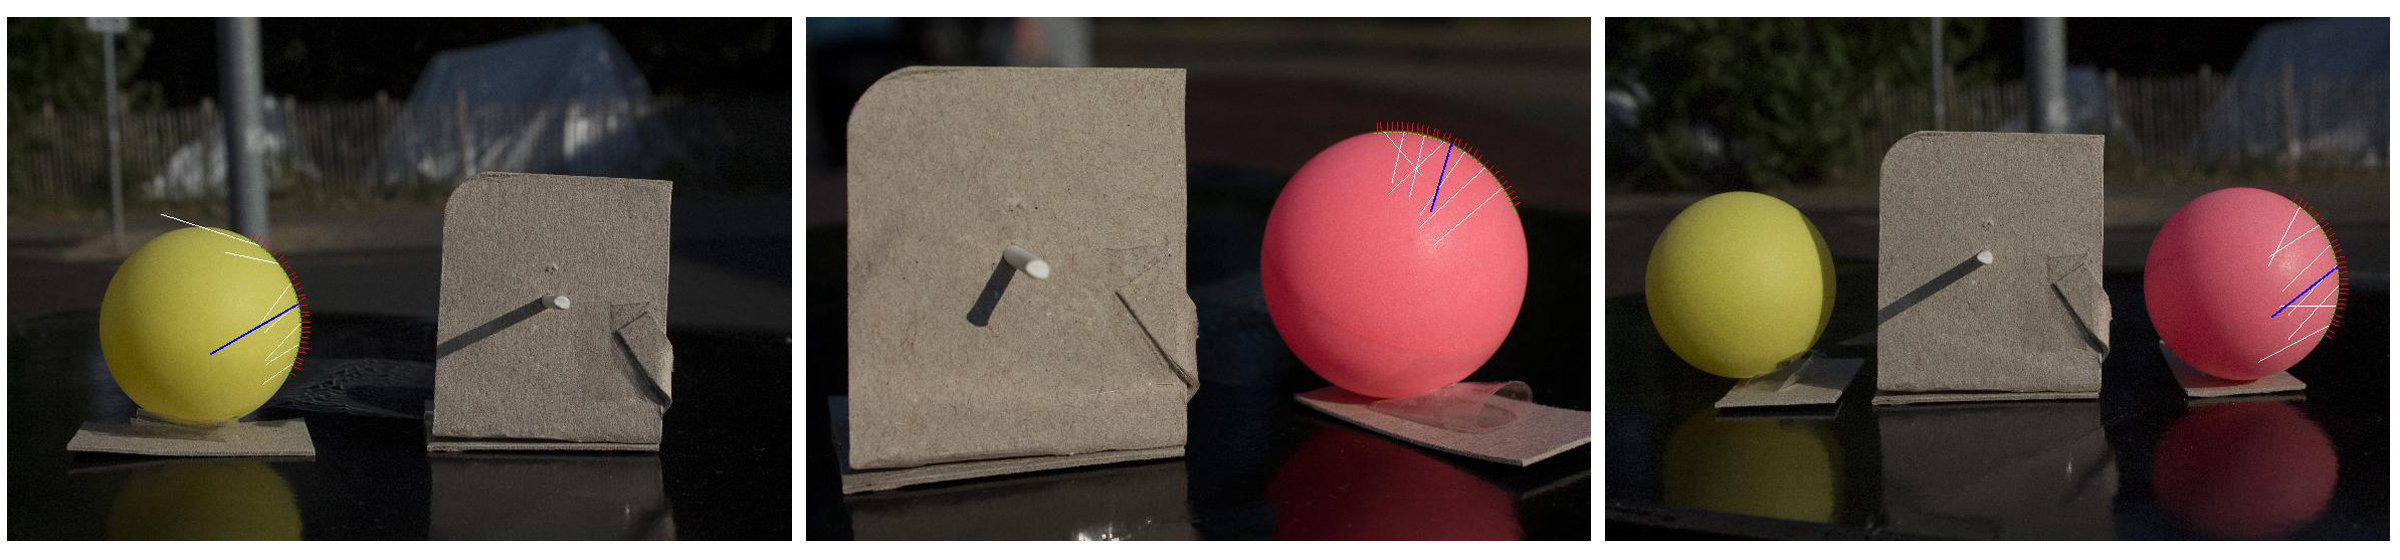
\includegraphics[width=\linewidth]{Images/Korrekte_Lightvectoren.jpg}	
	\caption[Bildunterschrift]{Correct estimated light vectors.}	
		\label{fig:goodRes}	
\end{figure}
Even so most of the approximated light vectors $\vec{v}$ are despite the few mentioned correct ones significantly wrong. Figures~\ref{fig:difDistance} and \ref{fig:divLightDirect} show that the patch light vectors $\vec{L}^n$ are not coherent and thus $\vec{v}$ points in the wrong direction as well. It is obvious that the norm of $\vec{v}$ does not fit to the length of the sun clock shadow. All estimation errors appear to be randomly and no correlations can be determined. 

To consider those correlations, the second batch of test images is split into two groups. The first part contains images that are captured with increasing distances (see Figure~\ref{fig:difDistance}). In comparison, the quality of the results turned out to be almost similar to the general observation and the coherence is still given. Thus, it can be assumed that the size of image section has no influence to the estimation error. 
\begin{figure}[H] 

	\center 
	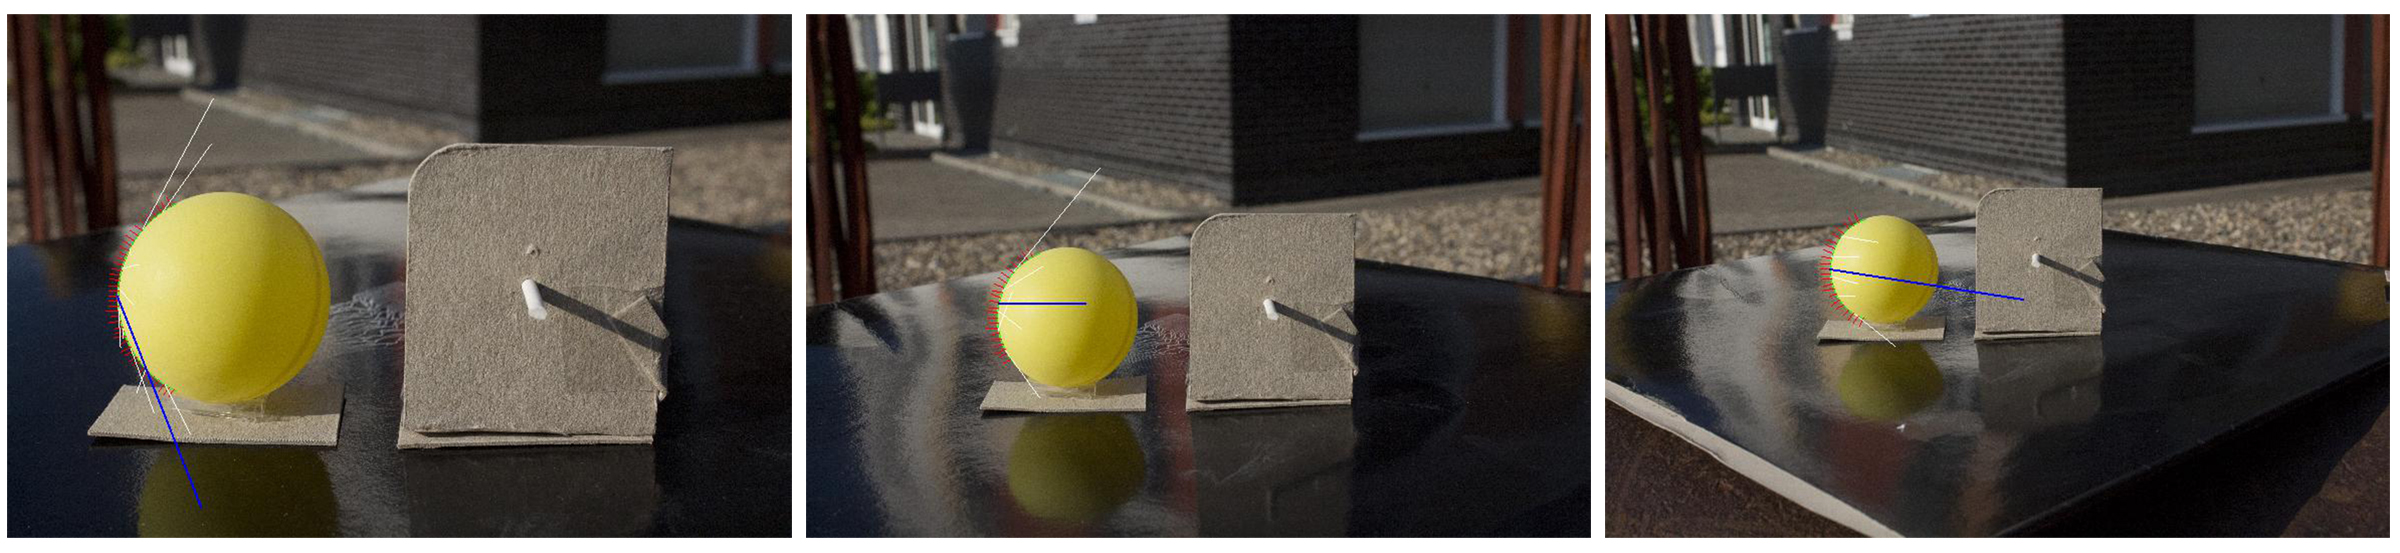
\includegraphics[width=\linewidth]{Images/versch_Anstaende.jpg}
	\caption[Bildunterschrift]{Results of images with increasing distances.}
		\label{fig:difDistance}		
\end{figure}
The second part includes images with various light direction to consider if the Johnson approaches has problems with special circumstances like the angle between $\vec{N}$ and $\vec{L}$ or a certain light directions. In Figure~\ref{fig:divLightDirect} is a collection of some examples out of this group shown. It gives the assumption that the algorithm is correctly implemented because the coherence is in the same range than with the general results. No significantly differences can be figured out related to certain light directions or angles and thus it can be assumed that the least square problem is correctly implemented and the high error rate is related to external influences like image noise, surface reflections and a huge ambient light proportion.
\begin{figure}[H] 

	\center 
	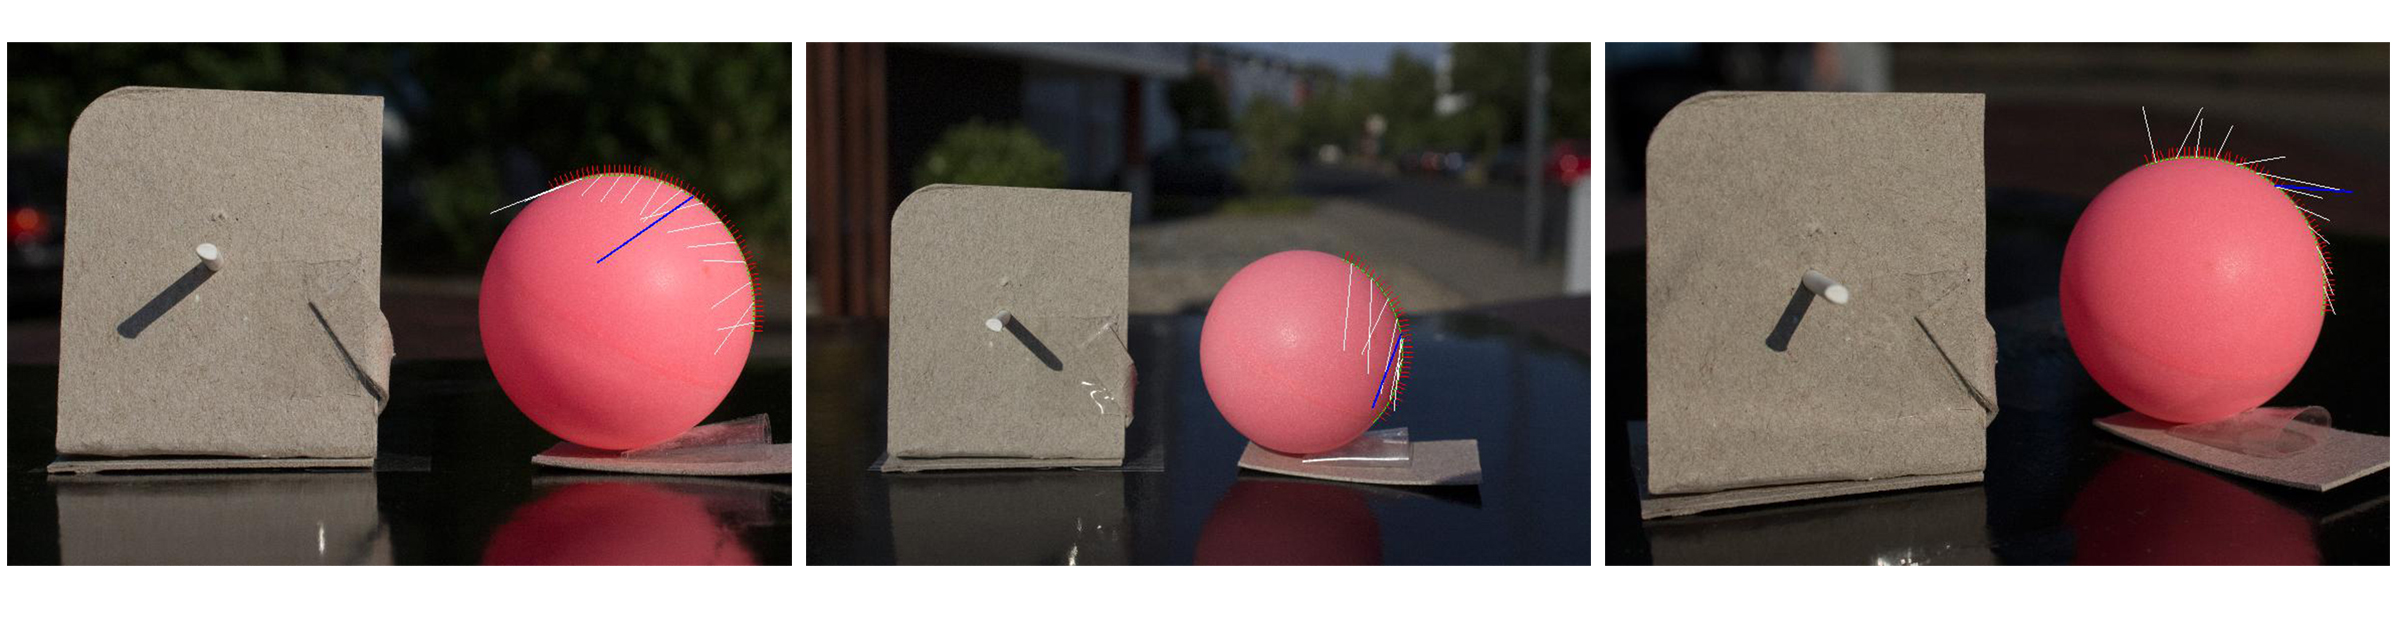
\includegraphics[width=\linewidth]{Images/versch_Lichtrichtungen.jpg}
	\caption[Bildunterschrift]{Results of images with various light directions.}
		\label{fig:divLightDirect}		
\end{figure}

This assumption is affirmed by the observation of the sub-contour position influence. The best results can be generated if the sub-contour fits closely and symmetrically around patch with highest intensity as in Figure~\ref{fig:goodRes}. Nonetheless, the success is quite sensible as shown in Figure~\ref{fig:subcontourRes}. Slightly variances in the length and position of the sub-contour results in significant changes of the direction and length. This proofs that correct results seems to be occasional and can not be forced by user intervention. 

\begin{figure}[H] 

	\center 
	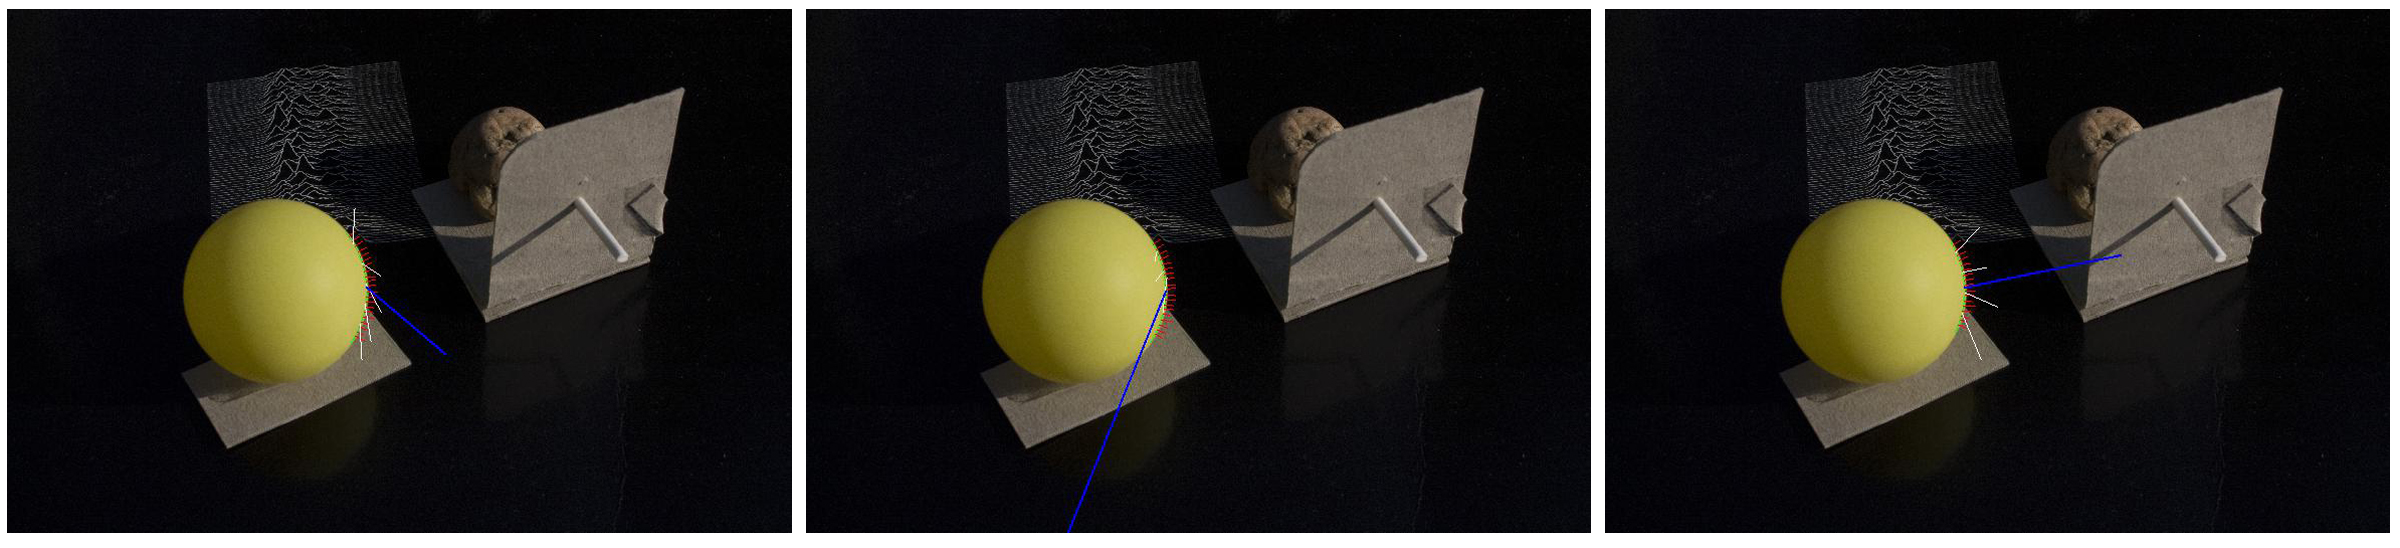
\includegraphics[width=\linewidth]{Images/Lage_der Subcontour.jpg}
	\caption[Bildunterschrift]{Results of slightly different sub-contours.}	
		\label{fig:subcontourRes}	
\end{figure}

The more complex objects of the second batch are evaluate as well and displayed in Figure~\ref{fig:complexRes}. Here, the image show obviously the randomness of the estimated vectors. Especially at the points where the contour changes significantly the direction, the $\vec{L}^n$ seems to have extremely wrong estimations but those outliers can be recognised in the other mentioned figures as well. Hence, the shape of the sub-contour seems to have no influence to the quality and robustness of this approach.
\begin{figure}[H] 
	
	\center 
	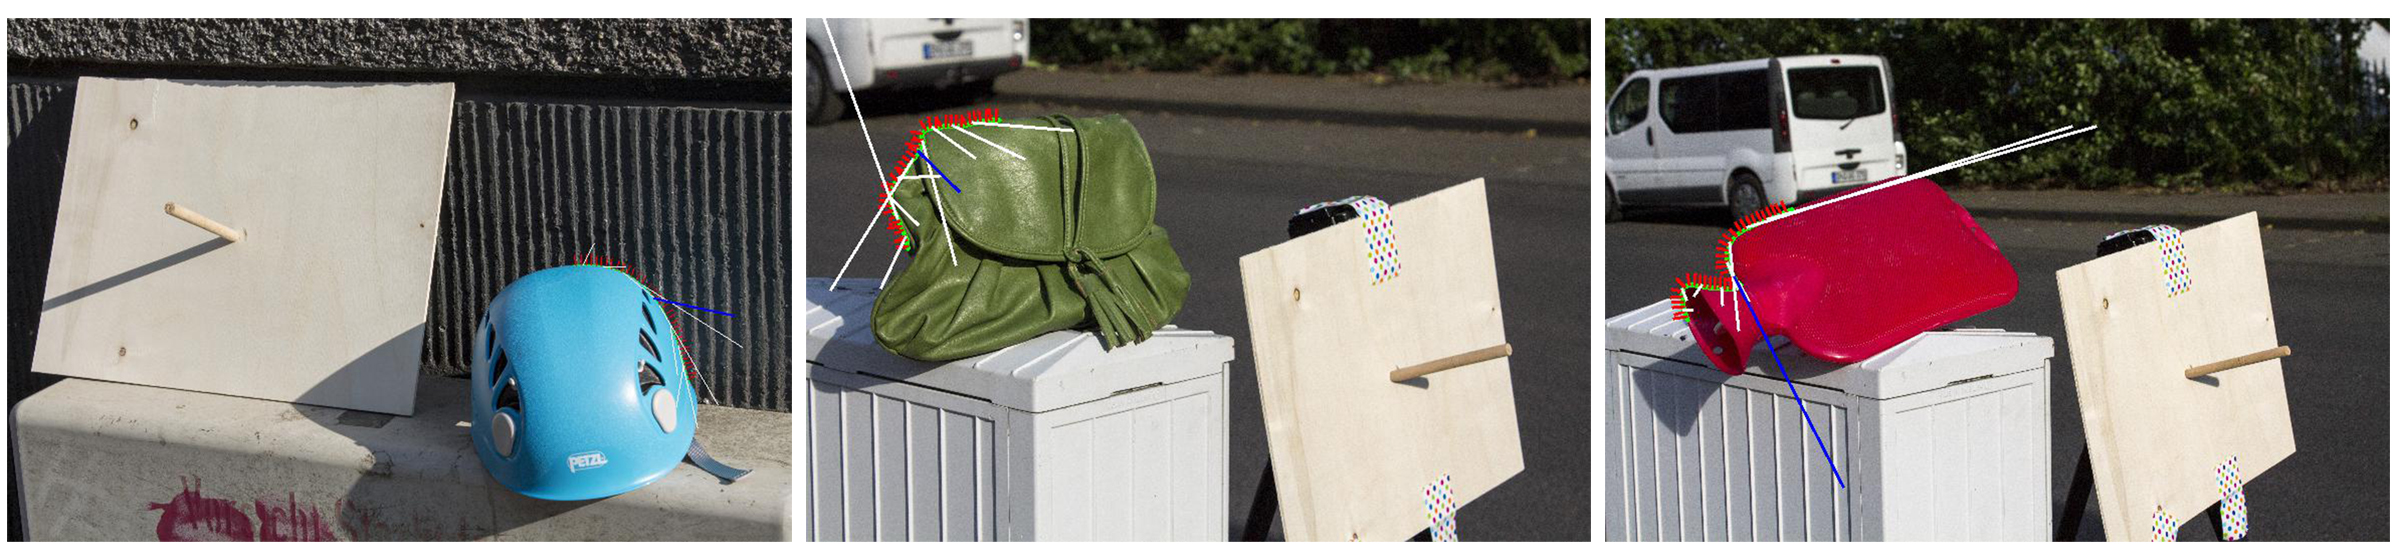
\includegraphics[width=\linewidth]{Images/Komplex_res.jpg}
	\caption[Bildunterschrift]{Results of more complex objects.}	
	\label{fig:complexRes}	
\end{figure}



\subsection{Evaluation 3. Approach}
Figure~\ref{fig:highRes} displays the results with the third approach which sets the light vector estimation $\vec{L}^max$ of the patch with the maximum intensity as $\vec{v}$. The direction seem to be as randomly as the results of the second approach and lacks of robustness and continuity. Even the $\vec{L}^n$ of the first batch images point in various direction with no coherence and the significant outliers at contour points where the direction changes can be recognised. In case of the lower left image an almost correct light vector could be approximated as well. These assumptions yields  that there are no significant differences in quality and trustworthiness between both approaches.
\begin{figure}[H] 
	\center 
	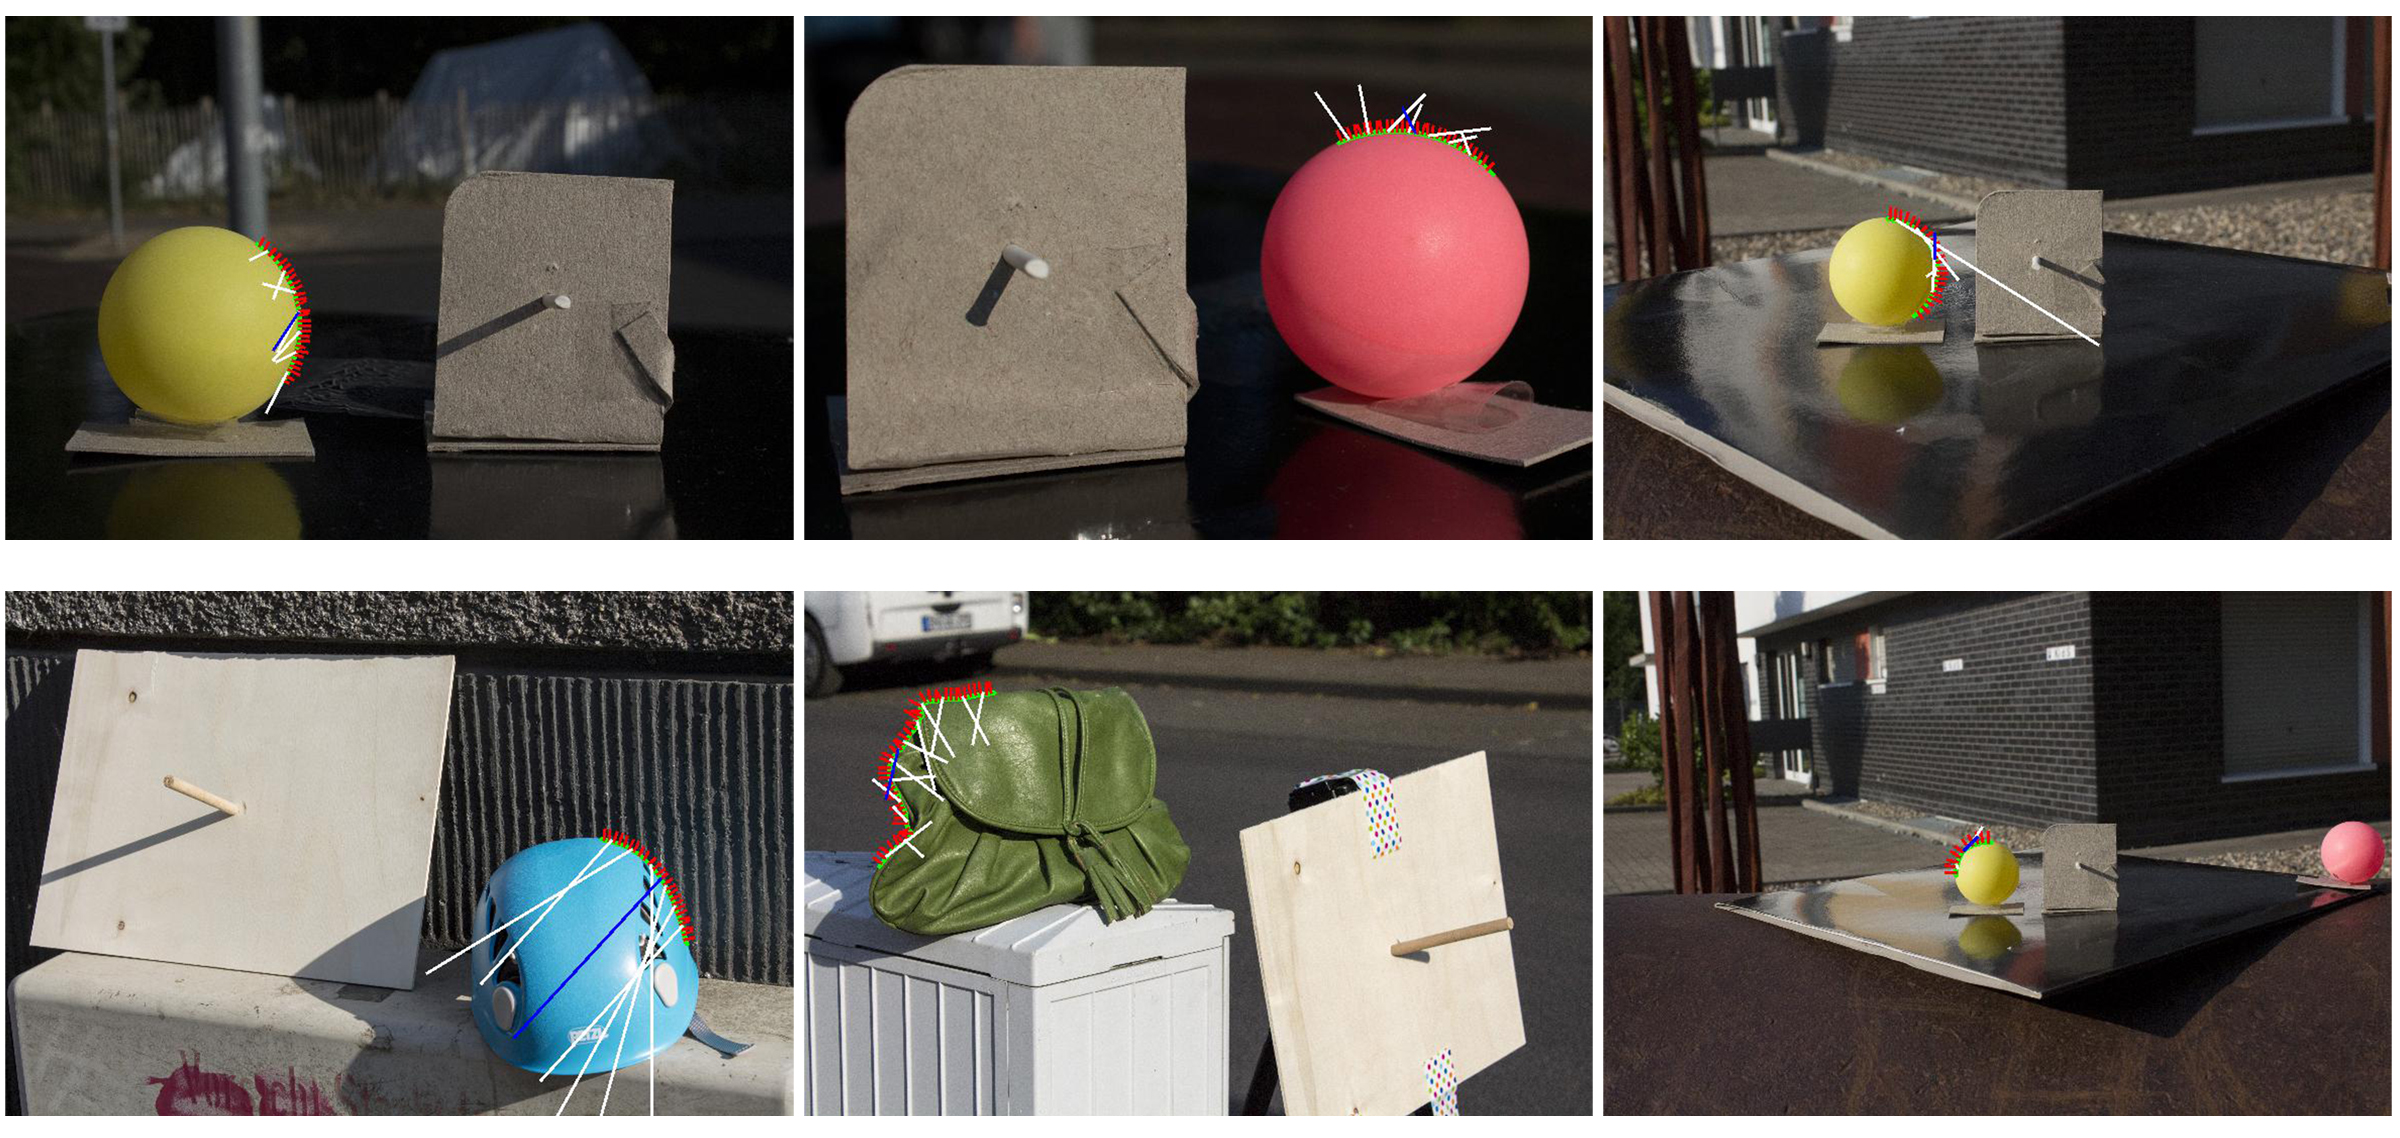
\includegraphics[width=\linewidth]{Images/High_res.jpg}
	\caption[Bildunterschrift]{Results of third approach with the light vector of the patch of highest intensity.}	
	\label{fig:highRes}	
\end{figure}
\subsection{Discussion of Evaluation Results}
The first assumption is to state the the current surface reflects light isotropically. This surface has a constant reflectance value $r$ and is illuminated by a faraway infinitive light source. Finally, the angle between $\vec{n}$ and  $\vec{l}$ is in the range of $0^\circ $ and $90^\circ$.


\begin{itemize}
	\item es ist auffällig, dass die autoren bei den Komplexeren Aufnahmen (mit den Promis) keine einzelne Lichtvekoren mehr einzeichnen. 
	\item Es wurde versucht möglichst homogene Objekte zum testen zu nehmen (vor allem der zweite Satz der Testbilder)
\end{itemize}

Beobachtungen unserer Versuche:\\
\begin{itemize}
	\item lediglich eine visuelle Auswertung
	\item Wir bekomen immer wieder Vektoren, die in die richtige Richtung zeigen  (bzw. um 180 gedrehte Vektoren) aber der Algorihtmus funtkioniert nicht zuverlässig
	\item Da Ergebnisse eher zufällig wirken, macht es keinen Sinn die drei Ansätze direkt miteinander zu vergleichen, der zweite Ansatz scheint jedoch am häufigste richtig zu liegen.
\end{itemize}

\subsection{Conclusion of Evaluation}







no difference of quality between more complex objects 
and ideal round objects

Conclusion: 
Algorithm of Johnson seems to be not reliable
Reflections and other light sources distort the result
Measuring the intensity is not sufficient
Assumptions of Johnson are not necessarily fulfilled in reality
Subcontour could exclude point with highest intensity



\newpage